%\documentclass[handout]{beamer}
\documentclass{beamer}
\mode<article>
{
	\usepackage{amscd}
	\usepackage{times,amsmath,amsbsy,amssymb,amsfonts,epic,hyperref}
	\usepackage[pdftex]{geometry}
	\usepackage[pdftex]{graphicx}
	\usepackage{fullpage}
	\usepackage{hyperref}
}

%\mode<presentation> {
%\usetheme{Madrid}
%\usecolortheme{dolphin}
%\usecolortheme{rose}
%}
\usepackage{amsfonts,bm,mathrsfs,subfig}
%\usepackage{movie15}

\mode<presentation> {
	\setbeamertemplate{background canvas}[vertical shading][bottom=red!10,top=blue!10]
	\usetheme{Boadilla}
	\usefonttheme[onlysmall]{structurebold}
}

\usepackage{multimedia}
\usepackage{animate} %need the animate.sty file

\usepackage{pgf,pgfarrows,pgfnodes,pgfautomata,pgfheaps,pgfshade,multirow}
\usepackage{amscd}
\usepackage{amsmath,amssymb}
%\usepackage[latin1]{inputenc}
\usepackage{colortbl}
\usepackage[english]{babel}
\usepackage{times}
\usepackage[T1]{fontenc}
\usepackage{epsf}
\usepackage{epsfig}
\usepackage{graphicx}
\usepackage{bm}
\usepackage{relsize}
\usepackage{dsfont}
\usepackage{pifont}
\usepackage{comment}
\usepackage{booktabs}
\newtheorem{algorithm}{Algorithm}
\newtheorem{remark}{Remark}
\usepackage{undertilde}
\usepackage{fancybox}
\usepackage{CJK}
\usepackage{multirow}
\usepackage{tikz}
\usepackage{slashbox}

%\input{mydef}
\def\p{\partial}
\def\u{{\mathbf u}}
% \def\B{{\mathbf B}}
\def\v{{\mathbf v}}
\def\n{{\mathbf n}}
% \def\F{{\mathbf F}}
%\def\A{{\mathbf A}}
% \def\x{{\mathbf x}}
\def\DD{\displaystyle}

\newcommand*{\ucong}{\mathrel{\text{\raisebox{.25ex}{\rotatebox[origin=c]{180}{$\cong$}}}}}
\newcommand{\relu}{\mbox{{\rm ReLU}}}



\newcommand{\red}[1]{\textcolor{red}{#1}}
\newcommand{\blue}[1]{\textcolor{blue}{#1}}
\newcommand{\brown}[1]{\textcolor{brown}{#1}}
\newcommand{\green}[1]{\textcolor{green}{#1}}


\newtheorem{prop}{Proposition}
\newtheorem{thm}{Theorem}
\newtheorem{prob}{Problem}
\newtheorem{assumption}{Assumption}
\newtheorem{defn}{Definition}
\newtheorem{coro}{Corollary}
\beamertemplatenavigationsymbolsempty


\newcommand{\tabincell}[2]{\begin{tabular}{@{}#1@{}}#2\end{tabular}}  

\newif\iflattersubsect

\AtBeginSection[] {
	\begin{frame}<beamer>
	\frametitle{Outline} %
	\tableofcontents[currentsection]  
\end{frame}
\lattersubsectfalse
}

\AtBeginSubsection[] {
\iflattersubsect
\begin{frame}<beamer>
\frametitle{Outline} %
\tableofcontents[currentsubsection]  
\end{frame}
\fi
\lattersubsecttrue
}

\begin{document}

\begin{CJK*}{UTF8}{gbsn}


\title[DNN \& FEM]
{Deep Neural Networks}

\author[Xu]{Jinchao Xu}

\institute[PSU]
{Penn State University\\[0.2cm]
	{\color{blue}\tt xu@math.psu.edu \;\; http://www.math.psu.edu/xu/}
}

\date[PSU]{Penn State \\ January 8, 2019}

\begin{frame}
\titlepage

{\footnotesize
	\centerline{Acknowledgement: }
	\centerline{{\color{blue} NSF Grants}: DMS-1522615 ~ DMS-1217142}
	\centerline{{\color{blue} DOE Grants}: DE-SC0014400 ~ DE-SC0009249}
}
\end{frame}


\begin{frame}
\frametitle{Outline} 
\setcounter{tocdepth}{2}
\tableofcontents
\end{frame}

\section{Supervised learning for classification problem}
%\subsection{Deep neural networks and its relation to FEM}
\begin{frame}{A basic AI problem: classification}
\begin{itemize}
	\item Can a machine (function) tell the difference ?
\end{itemize}

\begin{figure}
	\begin{center}
		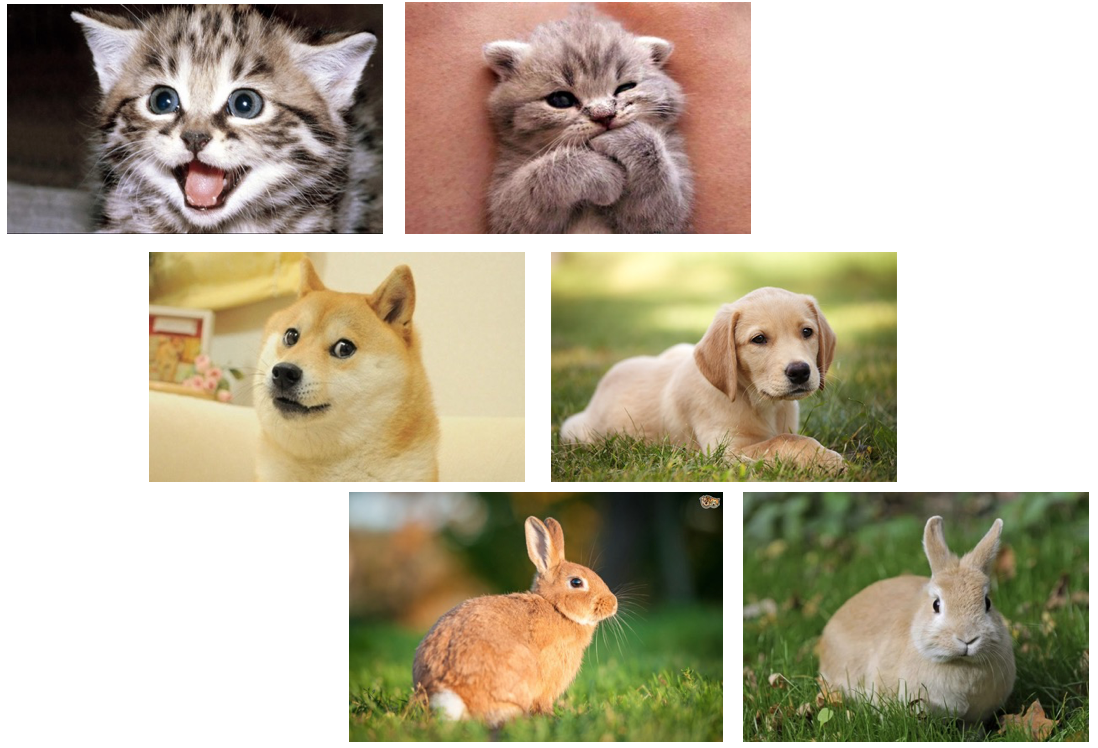
\includegraphics[width=.7\textwidth, height=.6\textheight]{figures/DL/cat-dog-1.png} 
	\end{center}
\end{figure}

\end{frame}

\begin{frame}{Supervised learning $\leftrightarrow$ Function interpolation}
\begin{itemize}
\item Each image = a big vector of pixel values 
\begin{itemize}
	\item $d=1280\times720\times3$ (width$\times$ height $\times$ RGB channel) $\approx$ 3M. 
\end{itemize}
\pause 
\item 3 different sets of points in $\mathbb{R}^d$, are they separable?
\begin{figure}
	\begin{center}
		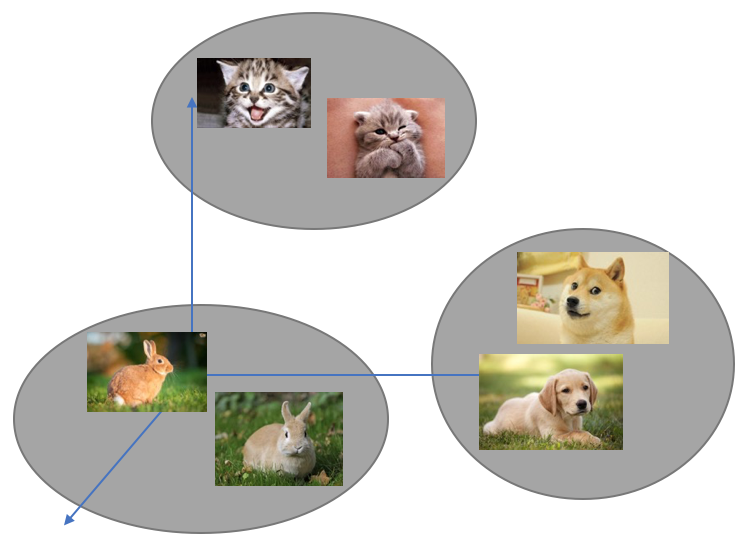
\includegraphics[width=.3\textwidth, height=.3\textheight]{figures/DL/cat-dog-2.png}   \quad \quad  \quad \quad 
		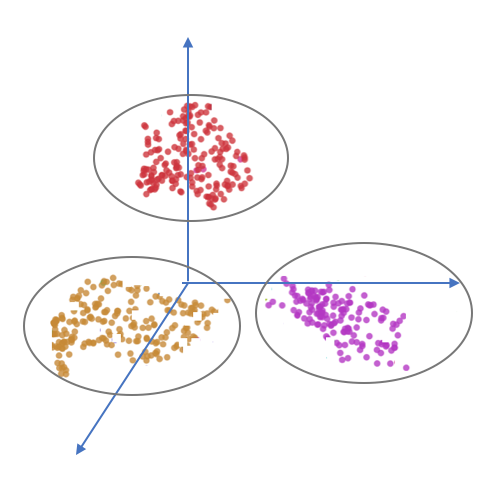
\includegraphics[width=.3\textwidth, height=.3\textheight]{figures/DL/cat-dog-3.png}  
	\end{center} 
\end{figure}
\pause 
\item Mathematical problem: Find $f(\cdot; \Theta): \mathbb{R}^d \to \mathbb{R}^3$ such that:
$$
f(
\includegraphics[width=.07\textwidth]{figures/DL/cat.png}; \Theta)
\approx \begin{pmatrix}
1\\ 0 \\ 0 
\end{pmatrix} 
\quad 
f(
\includegraphics[width=.07\textwidth]{figures/DL/dog.png}; \Theta)
\approx \begin{pmatrix}
0\\ 1 \\ 0 
\end{pmatrix} 
\quad 
f(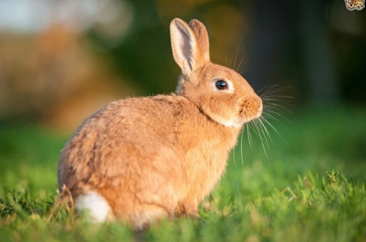
\includegraphics[width=.07\textwidth]{figures/DL/rabbit.png};
    \Theta) \approx 
\begin{pmatrix}
0\\ 0 \\ 1
\end{pmatrix} 
$$
\end{itemize}
\end{frame}

\begin{frame}
\frametitle{How to formulate ``learning''?}
\pause
\begin{itemize}
	\item Data: $\{x_i, y_i\}_{i=1}^m$
%%	\begin{itemize}
%%		\item Image Classification: $x_i$ image, $y_i$ object class
%%		\item Speech Recognition: $x_i$ audio, $y_i$ text
%%		\item Face Recognition: $x_i$ graph with face, $y_i$ identity
%%		\item ...
%%	\end{itemize}
\pause
	\item Find $f^*$ in some function class such that $f^*(x_i) \approx y_i$.
\pause
	\item Mathematically: solve the \red{optimization problem} by parameterizing the abstract function class
	\begin{equation}\label{eq:supervise}
	\min_{\Theta} L(x,y,\Theta)
	\end{equation}
where 
{\footnotesize
$$
L(x,y,\Theta)=
{\mathbb E}_{(x,y)\sim \mathcal D}[L(f(x; \Theta), y)]\approx
\frac{1}{m} \sum_{i=1}^m\|f(x_i; \Theta) - y_i\|^2
$$
}

\item Nonlinear least squares problems.
\end{itemize}
\end{frame}

\begin{frame}
  \frametitle{Main question}

\begin{quote}\large
 What is a good function class for $f$?    
\end{quote}

  
\end{frame}

\begin{frame}
\frametitle{What is a good function class for $f$?}
\begin{small}
\structure{Traditional machine learning models}
\begin{itemize}
\item linear regression 
\item  ``nonlinear" regression, 
\begin{itemize}
\item linears, polynomials, exponentials,  logarithms, trigonometric, ...
\end{itemize}
\pause 
\item SVM, decision tree...
	$$
	f(x;\Theta) = \sum_{k=1}^N c_k k(x,x_k).
	$$
\end{itemize}
\pause 
\structure{Traditional models in scientific  computing}
\begin{itemize}
	\item finite element methods, wavelets, spectral method ...
\end{itemize}
\end{small}
\end{frame}
\begin{frame}
{Challenges}
\begin{itemize}
	\item high dimension: image, video...
	\item big data: ImageNet, MegaFace...
	\item complex task: Go, auto-drive...
\end{itemize}
\end{frame}

\section{Deep neural networks}

\begin{frame}
  \frametitle{Linears, activation and composition}
\tiny
\pause 
\begin{enumerate}
\item Start from a linear function
$$
W^0x+b^0
$$
\pause 
\item Introduce an activation function $\sigma={\rm ReLU}(x)=\max(0,x)$:
	\begin{center}
		\includegraphics[width=.2\textwidth, height=.15\textheight]{figures/DL/ReLU.png} 
	\end{center}
\pause 
\item Compose with the activation function:
$$
x^{(1)}  = \sigma(W^0x+b^0)
$$
\pause 
\item Compose with another linear function:
$$
W^1x^{(1)}+b^1
$$
\pause 
\item Compose with the activation function:
$$
x^{(2)}=\sigma(W^1x^{(1)}+b^1)
$$
\pause 
\item Compose with another linear function
$$
f(x;\Theta)= W^2x^{(2)}+b^2
$$
\pause 
\item $\ldots$
\end{enumerate}
\end{frame}
\begin{frame}
\frametitle{Deep neural network functions}
DNN function class with super-parameters $\mathcal{N} = (n^1,\cdots,n^J)$: 
\begin{equation}\label{key}
{\rm DNN}_{J}({\mathcal{N}}) := \{f:\mathbb R^d\mapsto \mathbb R ~:~ f(x; \Theta) = f^J, \Theta \in \mathbb{R}^{\mathcal{N}}\}
\end{equation} 
where, with $\Theta=\Theta^J$ and $\Theta^j=(\Theta^{j-1},\theta^j)$, 
\pause
\begin{itemize}
	\item Recursion: $f^j(x,\Theta^j) = (\theta^j\circ \sigma \circ
	f^{j-1})(x,\Theta^{j-1}), \quad j=1:J$
\pause 
	\item Linear mapping: 
	$
	\theta^j: \mathbb{R}^{n^j} \to \mathbb{R}^{n^{j+1}} \quad \text{as} \quad \theta^j(x) =  W^j x + b^j,
	$
\pause 
	\item Initial: $f^0(x)=\theta^0(x).$
\pause 
	\item \red{nonlinear activation}:  $\sigma: \mathbb{R} \to \mathbb{R}$.   The
	popular one is ${\rm ReLU}(u)=\max(0,u)$:
\end{itemize}
\end{frame}




\begin{frame}
\frametitle{Approximation property of ${\rm DNN}_1$}
\small
One hidden layer ${\rm DNN}_1(N)$:
$$
f=\sum_{i=1}^N a_i\sigma(w_i\cdot x+b_i)
$$
\pause 
\structure{Question}
\begin{quote}
Is this function class rich enough to approximate any reasonable
(say, continuous) function?
\end{quote}
\pause 
\structure{Answers:}
\begin{enumerate}
\item  NO, if $\sigma$ is a polynomial 
\pause
\item  YES, if $\sigma$ is NOT a polynomial!
\end{enumerate}
\pause
\vfill
{\tiny M. Leshno, V. Lin, A. Pinkus and S. Schocken, 1993}
\end{frame}

\begin{frame}
  \frametitle{Special function class}
\structure{Special function class}
  \begin{quote}
Linears and composition with $1$  variable functions.
  \end{quote}
\pause
\structure{Approximation: any continuous function}
$$
f(x_1,\ldots,x_d)\sim \sum_{i=1}^N a_i\sigma\left(\sum_{p=1}^dw_i^px_p+b_i\right)
$$
\pause
\structure{Exact representation: any continuous function} [{\tiny
  Kolmogorov-Arnold 1957, Sprecher 1965}]
$$
f(x_1,\ldots,x_d)=\sum_{q=0}^{2d}\alert{\chi_f}\left(\sum_{p=1}^d\lambda^p\alert{\psi}(x_p+\epsilon
  q)+q\right).
$$
\pause
\structure{Disprove: Hilbert 13 problem}
\begin{quote}\tiny 
	Impossibility of the solution of the general equation of the 7th degree by means of functions of only two arguments.
\end{quote}
\end{frame}

\section{ReLU DNN and Linear Finite Elements}
\begin{frame} 
{What does a function in ${\rm DNN}_{\mathcal N}$ look like?}
\blue{Obviously:}
$$
{\rm DNN}_{\mathcal N}=\mbox{\rm a space of continuous piecewise linear functions!}
$$
\vskip-40pt 
\pause
\begin{figure}
	\begin{center}
		%$(10, 10)$ $(20, 20)$ $ (40,40)$  
		\includegraphics[width=.3\textwidth]{figures/2to10to10to1.pdf}  
		\includegraphics[width=.3\textwidth]{figures/2to20to20to1.pdf}  
		\includegraphics[width=.3\textwidth]{figures/2to40to40to1.pdf}  
	\end{center} 
\end{figure}
\vspace{-20mm}
\begin{center}
	$(10, 10)$ \qquad\qquad\qquad  $(20, 20)$ \qquad\qquad \qquad $ (40,40)$  
\end{center}
\end{frame}

\begin{frame}
\frametitle{Some mathematical questions}
\begin{enumerate}
\item Connection with finite element methods 
\item Approximation properties
\item What's the optimal structure?
\item Is deeper better?
\item How to reduce the number of parameters?
\end{enumerate}
\end{frame}


\begin{frame}{How is ${\rm DNN}_{\mathcal N}$ compared with (adaptive) linear FEM?}
\begin{figure}%[htbp]
\centering
\begin{minipage}[t]{0.3\textwidth}
\centering
\includegraphics[width=.7\textwidth, height=.3\textheight]{figures/dnn_grid.png} 
\caption{$(40, 40)$}
\end{minipage}
\begin{minipage}[t]{0.3\textwidth}
\centering
\includegraphics[width=.7\textwidth, height=.3\textheight]{figures/fem.pdf}
\caption{Uniform Grid}
\end{minipage}
\begin{minipage}[t]{0.3\textwidth}
\centering
\includegraphics[width=.7\textwidth, height=.3\textheight]{figures/L-adaptive.pdf}
\caption{Adaptive Grid}
\end{minipage}
\end{figure}

%\pause
%Some answers:
%\begin{itemize}
%\item DNN seems to be at least as good as adaptive linear FEM!
%\pause
%\item Any linear finite element function can be written as a DNN with ReLU!
%\end{itemize}
\end{frame}

\begin{frame}{Connection of ReLU DNN and linear FEM}
\begin{theorem}[He, Li, X and Zheng 2018]
Not all linear FE functions can be represented by a
shallow neural network, namely 
$$
{\rm LFE}\not\subset {\rm DNN}_1.
$$
\end{theorem}

\pause
\begin{theorem}[He, Li, X and Zheng 2018]
Given a locally convex finite element grid ${\cal
T}_h$, any linear finite element function with $N$ degrees of
freedom, it can be written as a ${\rm DNN}_J$ with 
$$
J = 2+\lceil\log_2 d_h\rceil
\mbox{ and }
N_{\rm neurons}=\mathcal{O}(d_hN).
$$
where $d_h$ is the largest number of elements that share one vertex.
\end{theorem}

\end{frame}


\begin{frame}{MRDA: a sparse optimization method in Deep Learning}
\structure{Modified Regularized Dual Averaging (MRDA)}
\begin{itemize}
	\item 	Loss function with $\ell^1$ regularization term,
	\begin{equation}\label{regularized expected risk minimization}
	\min_{\Theta}~~\left\lbrace \phi(\Theta) =  \mathbf{E}_z f(\Theta,z)+\Psi(\Theta)\right\rbrace.
	\end{equation}
	\item 
	$$
	\Theta_{t+1} =\mathop{\arg\min}_\Theta \left\{\frac{1}{t} \sum_{\tau=1}^{t} \left<g_{\tau},\Theta \right>+\frac{\beta_t}{t}h(\Theta)+\Psi(\Theta)\right\}.
	$$
\end{itemize}
\vspace{2.5cm}
\vfill 
\tiny \structure{Ref:}  {L. Xiao 2010, X. Jia, L. Zhao, L. Zhang, J. He and J. Xu 2018}
\end{frame}

\begin{frame}\frametitle{MRDA: a sparse optimization method in Deep Learning}
%	\footnote{Jia, X., Zhao, L., Zhang, L., He, J., \& Xu, J. Modified Regularized Dual Averaging Method for Training Sparse Convolutional Neural Networks. \emph{arXiv preprint arXiv} arXiv:1807.04222, 2018}
\begin{theorem}[Jia, Zhao, Zhang, He and X 2018]\label{Convergence_Modified_RDA}
Assume there exists an optimal solution $\Theta^{\star}$ to the problem (\ref{regularized expected risk minimization}) for convex case with $\Psi(w)=\lambda\|\Theta\|_1$ that satisfies $h(\Theta^{\star})\leq D^2$ for some $D>0$, and let $\phi^{\star}=\phi(\Theta^{\star}).$ Let the sequences $\{\Theta_t\}_{t\geq 1}$ be generated by modified RDA method, and assume $\|g_t\|_{\ast}\leq G$ for some constant $G$. Then the expected cost $\mathbf{E}\phi(\bar{\Theta}_t)$ converges to $\phi^{\star}$ with rate $O(\frac{1}{\sqrt{t}})$
$$
\mathbf{E}\phi(\bar{\Theta}_t)-\phi^{\star}
= O(\frac{1}{\sqrt{t}}).
$$
\end{theorem}
\vspace{1.5cm}
\vfill 
\tiny \structure{Ref:}  {L. Xiao 2010, X. Jia, L. Zhao, L. Zhang, J. He and J. Xu 2018}
\end{frame}

\begin{frame}
\frametitle{Numerical Results on CIFAR-10}
\begin{table}[H]
\centering
\caption{Different Methods on ResNet18. The models are trained for $120$ epochs. While the validation accuracies are close, proximal-SGD gives poor sparse solutions compared to MRDA, and SGD introduces no sparsity.}
\begin{tabular}{l rrr}
\hline\hline
Method & TOP 1 & TOP 5 & $\sigma$             \\ \hline
SGD    	  & 89.27 &	99.57 &	$0.00$      \\  
proximal-SGD  	  & 89.80 & 99.40 & $0.03$ \\
\red{MRDA}  	  & 90.67 &	99.53 &	\red{$0.94$}     \\  
[1ex]
\hline
\end{tabular}
\end{table}
\begin{equation}
\sigma = \frac{\text{number of zero parameters}}{\text{number of all parameters}}.
\end{equation}
\end{frame}

\begin{frame}
\frametitle{Numerical Results on CIFAR-10}
\begin{table}[H]
\centering
\caption{RDA on different architectures. The models are trained for $120$ epochs. The results from SGD with momentum are in the brackets. }
\begin{tabular}{l|rrrrr}
\hline\hline
Architecture & TOP 1 & TOP 5 & $\sigma$             \\ \hline
VGG16  	  & 89.01 (93.42) & 99.36 (99.79) & \red{$0.76$}  \\
ResNet18  & 90.67 (89.27) &	99.53 (99.57) &	\red{$0.94$}  \\
VGG19     & 89.50 (91.70) &	99.21 (99.40) &	\red{$0.97$} \\
\hline
\end{tabular}
\end{table}
\end{frame}

\begin{frame}
\frametitle{Numerical Results on Different Datasets}
\begin{table}[H]
\centering
\caption{RDA on ResNet18 with different datasets. The models are trained for $120$ epochs, except for CIFAR-100, which is trained for 1900 epochs. The results from SGD with momentum are in the brackets.}
\begin{tabular}{l rrr}
\hline\hline
Dataset & TOP 1 & TOP 5 & $\sigma$   \\ \hline
MNIST   & 99.63 (99.65) & 100.00 & \red{0.95}    \\
CIFAR-10 & 90.67 (89.50) & 99.53 (99.21) &	\red{0.94}  \\
CIFAR-100 & 72.29 (73.69) & 89.94 (92.43) & \red{0.56}  \\
ImageNet & 63.13 (70.58) & 84.92 (89.64) & \red{0.36} \\ 
\hline
\end{tabular}
\end{table}
\end{frame}

\section{CNN  and Multigrid}
\begin{frame}{Convolutional Neural Networks (CNN)}
\begin{columns}
\begin{column}{0.6\textwidth}
CNN has been successfully used in:
\begin{itemize}
\item Computer vision
\begin{itemize}
\item Classification, detection, segmentation...
\item Medical image processing,
\item Face recognition,
\end{itemize}
\item Reinforcement learning
\begin{itemize}
\item AlphaGo,
\item Automated driving,
\end{itemize}
\item Natural language processing
\begin{itemize}
\item Speech recognition,
\item  Machine translation,
\end{itemize}
\item ...
\end{itemize}
\end{column}

\begin{column}{0.4\textwidth}
\centering  

\includegraphics[width=\textwidth, height= 0.4\textheight]{figures/ImageNet}  \\
\centering  
\includegraphics[width=\textwidth, height= 0.4\textheight]{figures/Alphago}  
\end{column}

\end{columns}

\end{frame}


\begin{frame}{Convolution operation in CNN}
\begin{tabular}{cc}
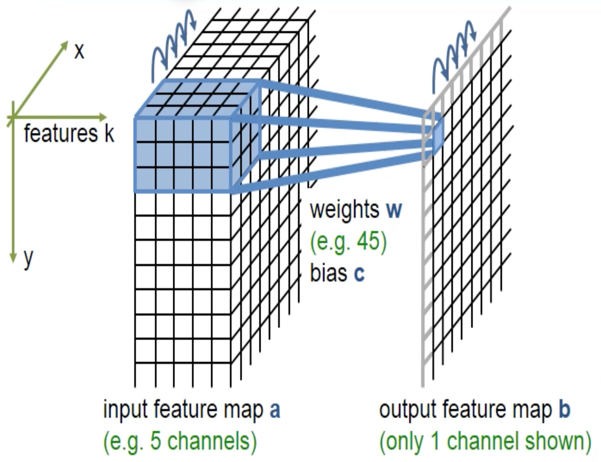
\includegraphics[width=0.45\textwidth]{figures/CNNLayer1} & 
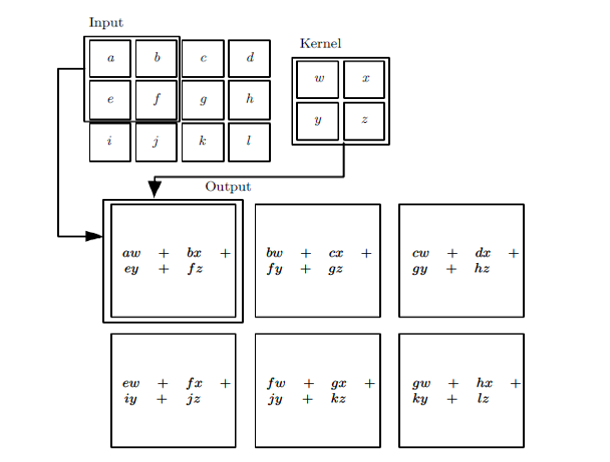
\includegraphics[width=0.45\textwidth]{figures/CNNLayer2}
\end{tabular}

\begin{equation}\label{eq:conv}
(K \ast x)_{i,j} :=\sum_{\ell=1}^c \sum_{s, t = -k}^k  K_{s+k+1,t+k+1,\ell} x_{i + s, j + t,\ell},
\end{equation}
\begin{itemize}
\item $i,j$: essential dimension
\item $\ell$: channel dimension
\end{itemize}
\end{frame}

\begin{frame}{Sub-sampling (coarsening): stride and pooling}
\begin{columns}
\begin{column}{0.5\textwidth}
\begin{center}
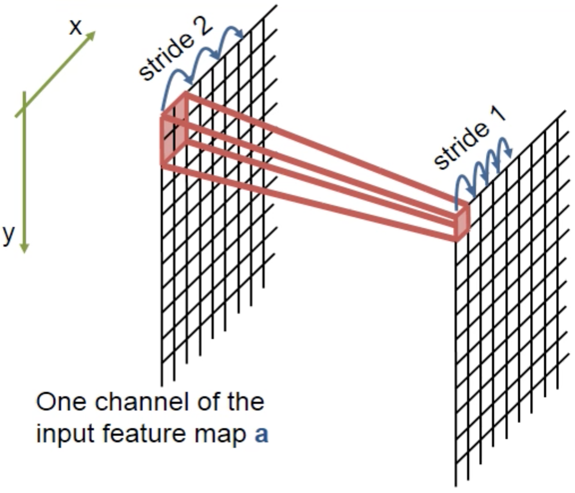
\includegraphics[width=.6\textwidth, height=0.4\textheight]{figures/PoolingLayer1} 
\end{center}
\begin{itemize}
\item Convolution with stride
{\tiny
$$(K\ast_{s} x)_{i,j} = \sum_{\ell=1}^c\sum_{p, q = -k}^k K_{p+k+1,q+k+1}x_{is + p, js + q} .$$
}
\end{itemize}
\end{column}
\begin{column}{0.5\textwidth}	
\begin{center}
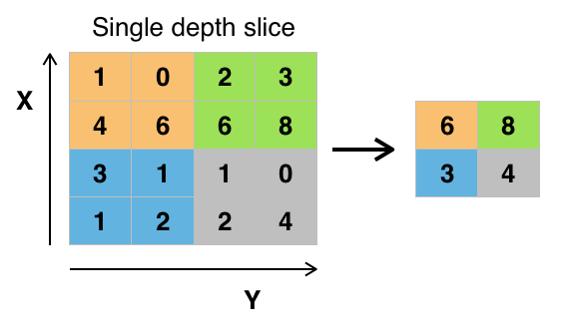
\includegraphics[width=.6\textwidth, height=0.4\textheight]{figures/PoolingLayer2}
\end{center}	
\begin{itemize}
\item Pooling (max-pooling)
{\tiny
$$r(x)_{i,j} = \max\{x_{(i-1)s + p,(j-1)s + q} ~:~ p,q = 1:s\}.$$
}
\end{itemize}
\end{column}
\end{columns}
\end{frame}


\begin{frame}{Fully-connected layers (DNN)}
\begin{columns}
\column{0.3\textwidth}  
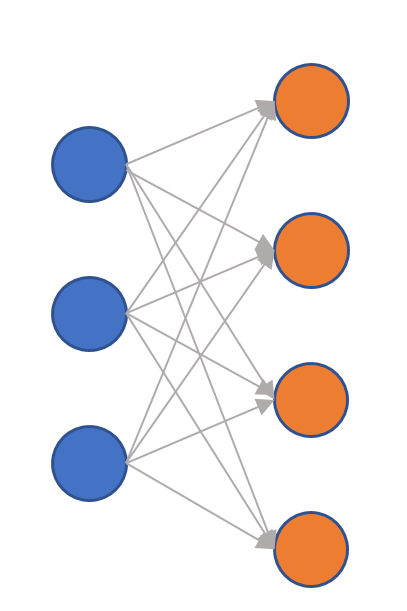
\includegraphics[width=\textwidth]{figures/FC}
\column{0.7\textwidth} % remember add this to the other clumn  
\begin{minipage}[c][0.45\textheight][c]{\linewidth} 
\begin{itemize}
\item Each neuron in the previous layer is connected with each neuron in the latter layer 
\item A fully-connected layer can be represented with the following linear function
$$y=Wx+b$$
\begin{itemize}
\item $x$ --- input
\item $y$ --- output
\item $W,b$--- parameters

\end{itemize}
\item Fully-connected layer makes classification with the features extracted by the convolutional layer

\end{itemize}

\end{minipage}
\end{columns}  
\end{frame}

\begin{frame}{A complete convolutional neural network example}
\begin{columns}
\column{0.25\textwidth}  
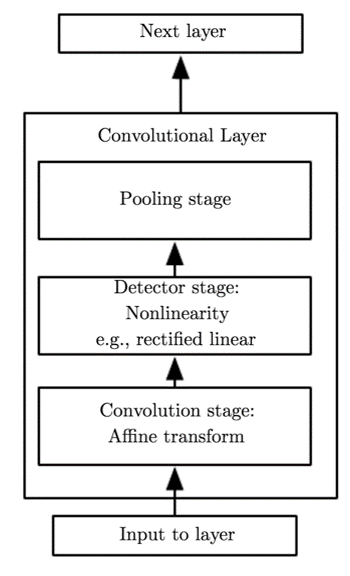
\includegraphics[width=\textwidth]{figures/CNN1}
\column{0.7\textwidth} % remember add this to the other clumn  
\begin{figure}
\begin{center} 
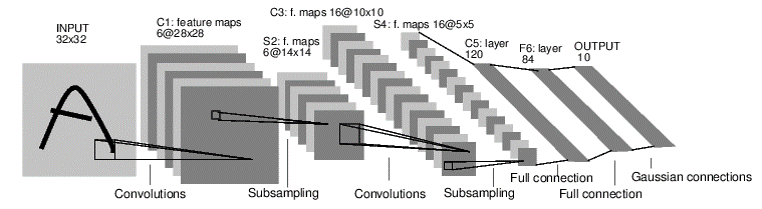
\includegraphics[width=\linewidth]{figures/CNN2}  
\caption{First convolutional neural network: LeNet-5 (Y. LeCun, L. Bottou, Y. Bengio, and P. Haffner, 1998)}
\end{center}
\end{figure} 
\begin{itemize}
\item Convolutional layer: extract the features of the graphs 
\item Fully-connected layer: make classification with the extracted features
\end{itemize}
\end{columns}  
\end{frame}


\begin{frame}{Deeper and better}
\begin{figure}
\begin{center}
\includegraphics[width=0.8\textwidth]{figures/Depth}
\end{center}
\caption{Depth in ImageNet \footnote{slide from Kaiming He's presentation}}
\end{figure}
\begin{itemize}
\item  { \blue{Questions:} Why CNN works? Is deeper always better? Why?}
\item Our idea: connection with \blue{multigrid methods}!
\end{itemize}
\end{frame}

\begin{frame}
\frametitle{{\small Convolutional Neural Networks and Multigrid
		Methods 
		\footnote{\blue{J. Xu}, Deep Neural Networks and Multigrid
			Methods ({L}ecture {N}otes at {P}enn {S}tate), 2017.}
		\footnote{\blue{J. He}, \blue{J. Xu}, Residual Structure in CNN and
			Multigrid Methods \textsl{in preparation, 2018}.}
} }
\begin{columns}
	\begin{column}{0.4\linewidth}
		\begin{itemize}
			\item Connection between ResNet and MG
			{\small
				\item Hierarchy level of ``grids''
				\item PDE-based model
				\item Residual structures
				\item Smoother \emph{vs.} Convolution
				\item Restriction \emph{vs.} Pooling
				\item Adaptivity \emph{vs.} Training
				\item ...
			} 
		\end{itemize}
	\end{column}
	\begin{column}{0.6\linewidth}
		\begin{figure}
			\begin{center}
				\includegraphics[width=.85\textwidth, height=.6\textheight]{figures/DL/Fig-CNN-MG.png}
			%	\caption{V-cycle \emph{vs.} ResNet}
			\end{center}
		\end{figure}
	\end{column}
\end{columns}
\end{frame}

\begin{frame}{MATH 597: Deep Learning}
\begin{description}
\item[Instructor] Professor Jinchao Xu, 314 McAllister Building, http://www.math.psu.edu/xu/
\item[Time] Tuesday and Thursday 12:05pm-1:20pm, 114 McAllister Building
\item[Office hours:] Tuesday and Thursday 3:00pm-4:00pm
\item[PREREQUISITE:]
A good knowledge of multi-variable calculus, linear
algebra and basic numerical analysis

\item[REQUIREMENT:  ]$\quad$

  \begin{itemize}
  \item Homework and programming assignments  (60\%) 
\item Take-Home Midterm (20\%) Take-Home Final (20\%).
  \end{itemize}
\item[REFERENCES:]  PDF files of detailed lectures notes will be available to
the  class.
\end{description}

\end{frame}
\begin{frame}
{Topics}
\begin{itemize}
\item Elements of probability and statistics
\item Basic theory of machine learning
\item Basic structure of deep neural networks
\item Approximation properties of DNN 
\item Convolutional neural networks
\item Recurrent neural networks
\item Generative Adversarial Networks
\item Stochastic gradient descent methods 
\item DNN and finite element methods
\item Multigrid methods
\item MgNet
\item Python
\item MNIST
\item TensorFlow, PyTorch
\end{itemize}
\end{frame}
\end{CJK*}


\end{document}
